\documentclass[b5paper,12pt,twoside,openright]{book}

\usepackage{amsmath}
\usepackage{graphicx}
\usepackage{caption}
\usepackage{verbatim}
\usepackage{float}
\usepackage{pgfplots}
\usepackage{subcaption}
\usepackage{fancyhdr}
\usepackage{caption}
\usepackage{datatool}
\usepackage{filecontents}
\usepackage[Lenny]{fncychap}
\restylefloat{table}
\title{Self-assembly mechanisms for evolutionary robotics}
\author{Eirik Jakobsen\\ Christopher Tannum}
\date{December 2015}

\usepackage[lmargin=25mm,rmargin=25mm,tmargin=27mm,bmargin=30mm]{geometry}

\newcommand{\insertresultgraphs}[4]{
	\ifodd\value{page}
		\begin{tikzpicture}[remember picture,overlay]
   			\node[anchor=south west,outer xsep=10pt, outer ysep=10] at (current page.south west)
         	{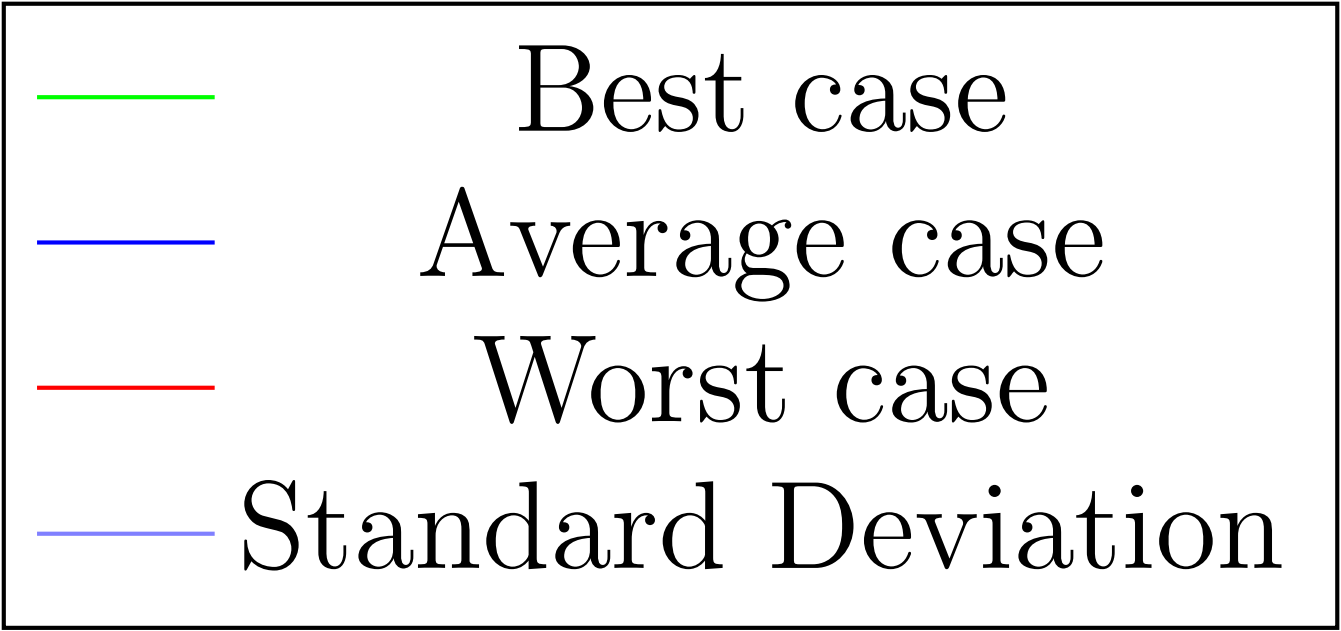
\includegraphics[scale=0.07]{chapters/res/generated_graph_legend.png}};
		\end{tikzpicture}
	\else%
		\begin{tikzpicture}[remember picture,overlay]
   			\node[anchor=south east,outer xsep=10pt, outer ysep=10] at (current page.south east)
         	{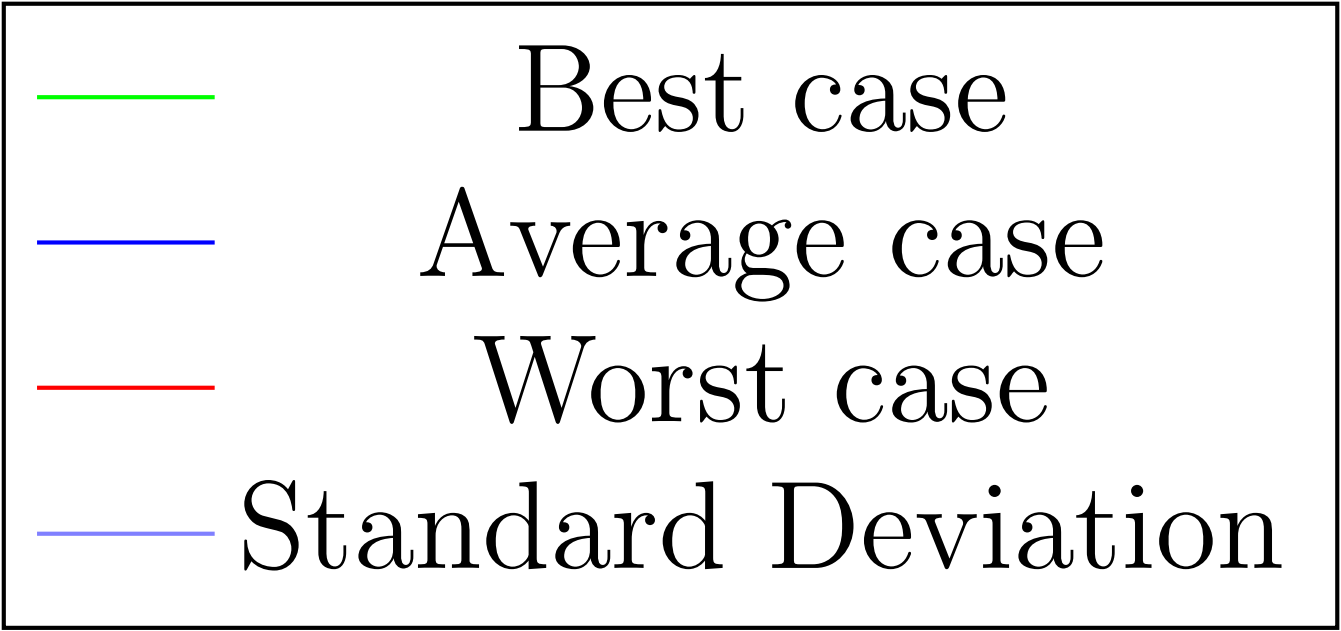
\includegraphics[scale=0.07]{chapters/res/generated_graph_legend.png}};
		\end{tikzpicture}
	\fi

	\begin{figure}[H]
		\makebox[\linewidth][c]{%
		\begin{subfigure}[b]{0.5\textwidth}
			\centering
			\resizebox{\linewidth}{!}{\input{#1}}
			\caption{\textbf{{\footnotesize 2-ports}}}
		\end{subfigure}%
		\begin{subfigure}[b]{0.5\textwidth}	
			\centering
			\resizebox{\linewidth}{!}{\input{#2}}
			\caption{\textbf{{\footnotesize 3-ports}}}
		\end{subfigure}%
	}
	\\
	\\
		\makebox[\linewidth][c]{%
		\begin{subfigure}[b]{0.5\textwidth}
			\centering
			\resizebox{\linewidth}{!}{\input{#3}}
			\caption{\textbf{{\footnotesize 4-ports}}}
		\end{subfigure}%
	}
	\caption{#4}
	\end{figure}

}


\fancypagestyle{main}{%
  	\fancyhead{}
	\fancyfoot{}
	\fancyfoot[LE,RO]{\thepage}

	\fancyhead[R]{\small\nouppercase\leftmark}
	\fancyhead[L]{\small\nouppercase\rightmark}

	\renewcommand{\footrulewidth}{0.4pt}
	\renewcommand{\headrulewidth}{0.4pt}
}

\fancypagestyle{start}{%
  	\fancyhead{}
	\fancyfoot{}
}

\fancypagestyle{plain}{%
  	\fancyhead{}
	\fancyfoot{}
  	\renewcommand{\headrulewidth}{0pt}
  	\renewcommand{\footrulewidth}{0.4pt}
  	\fancyfoot[LE,RO]{\thepage}
}

\DeclareCaptionType{captioneq}[][List of equations]
\captionsetup[captioneq]{labelformat=empty}

\begin{document}

\pagestyle{start}

\begin{titlepage}
    \begin{center}
    
    	\vspace{1cm}
		
		\large
		\textbf{TDT4501 Computer Science, Research Project\\}    
		
		\vspace{0.5cm}		
		
		\small    	
    	\textbf{Autumn 2015}
    	
        \vspace{5.2cm}
        
        \Huge
        \textbf{Self-assembly mechanisms for evolutionary robotics}
        
        \vspace{0.3 cm}
        
        \large
        Norwegian University of Science and Technology
        
        \vspace{4.5cm}
        
        
        \Large
        \textbf{Eirik Jakobsen\\ Christopher Tannum}
        
        \vspace{1cm}
        
        \small
        \textbf{Advisors:\\}
    	\textit{Jean-Marc Montanier \\ Kazi Shah Nawaz Ripon \\ Pauline Haddow}
    \end{center}
\end{titlepage}

\frontmatter
\pagestyle{plain}

\chapter*{
    \begin{center}
        Abstract
    \end{center}
}

\tableofcontents

\newpage

\mainmatter
\pagestyle{main}

\begin{center}
	\subsection{Robot Something}
	\vspace*{-0.7cm}
\end{center}




\insertresultgraphs{chapters/generated-graphs/2-ports/predators_eaten-out-2-ports.tex}{chapters/generated-graphs/2-ports/robots_eaten-out-2-ports.tex}{chapters/generated-graphs/2-ports/robots_starved-out-2-ports.tex}{Figure shows results from a 2 connection port simulation}

Lorem ipsum dolor sit amet, consectetur adipiscing elit. Pellentesque commodo tellus lorem, non sollicitudin diam commodo ut. Maecenas enim eros, bibendum a odio sed, finibus fermentum velit. In molestie orci non diam semper, in tempor nisl porta. Duis sodales elementum ornare. Quisque at lacus ac leo dictum finibus. Cras vel pretium risus, vel ornare erat. Morbi in elit non leo venenatis sodales at ut lectus. Fusce ac mollis nunc. Suspendisse aliquam molestie mauris, a molestie orci dictum sed. Fusce ac mollis nunc. Suspendisse aliquam molestie mauris, a molestie orci dictum sed. 

\end{document}